\section{Crowd Counting}
\subsection{Gaussian Kernels}

The most general form of a 2D Gaussian function, including rotation, is written as:
\[
f(x, y) = A \exp \left( -\left[ a(x - x_0)^2 + 2b(x - x_0)(y - y_0) + c(y - y_0)^2 \right] \right),
\]
where the coefficients \(a\), \(b\), and \(c\) define the shape and orientation of the elliptical contours. The associated matrix
\[
\begin{bmatrix}
a & b \\
b & c
\end{bmatrix}
\]
must be symmetric and positive-definite for the function to be a proper Gaussian. In this form, \(A\) still determines the peak amplitude, and \((x_0, y_0)\) is the center.

If the elliptical Gaussian is derived from an axis-aligned Gaussian that has been rotated by an angle \(\theta\), then the parameters \(a\), \(b\), and \(c\) are given by:
\[
\begin{aligned}
a &= \frac{\cos^2 \theta}{2\sigma_X^2} + \frac{\sin^2 \theta}{2\sigma_Y^2}, \\
b &= -\frac{\sin \theta \cos \theta}{2\sigma_X^2} + \frac{\sin \theta \cos \theta}{2\sigma_Y^2}, \\
c &= \frac{\sin^2 \theta}{2\sigma_X^2} + \frac{\cos^2 \theta}{2\sigma_Y^2}.
\end{aligned}
\]
These expressions correspond to a counterclockwise rotation by angle \(\theta\). A clockwise rotation can be achieved by negating the angle or flipping the sign of \(b\). \cite{wiki:gaussian}. Example of rotations of Gaussian blobs in image \textbf{\ref{fig:gauss}}

\begin{figure}[h]
    \centering
    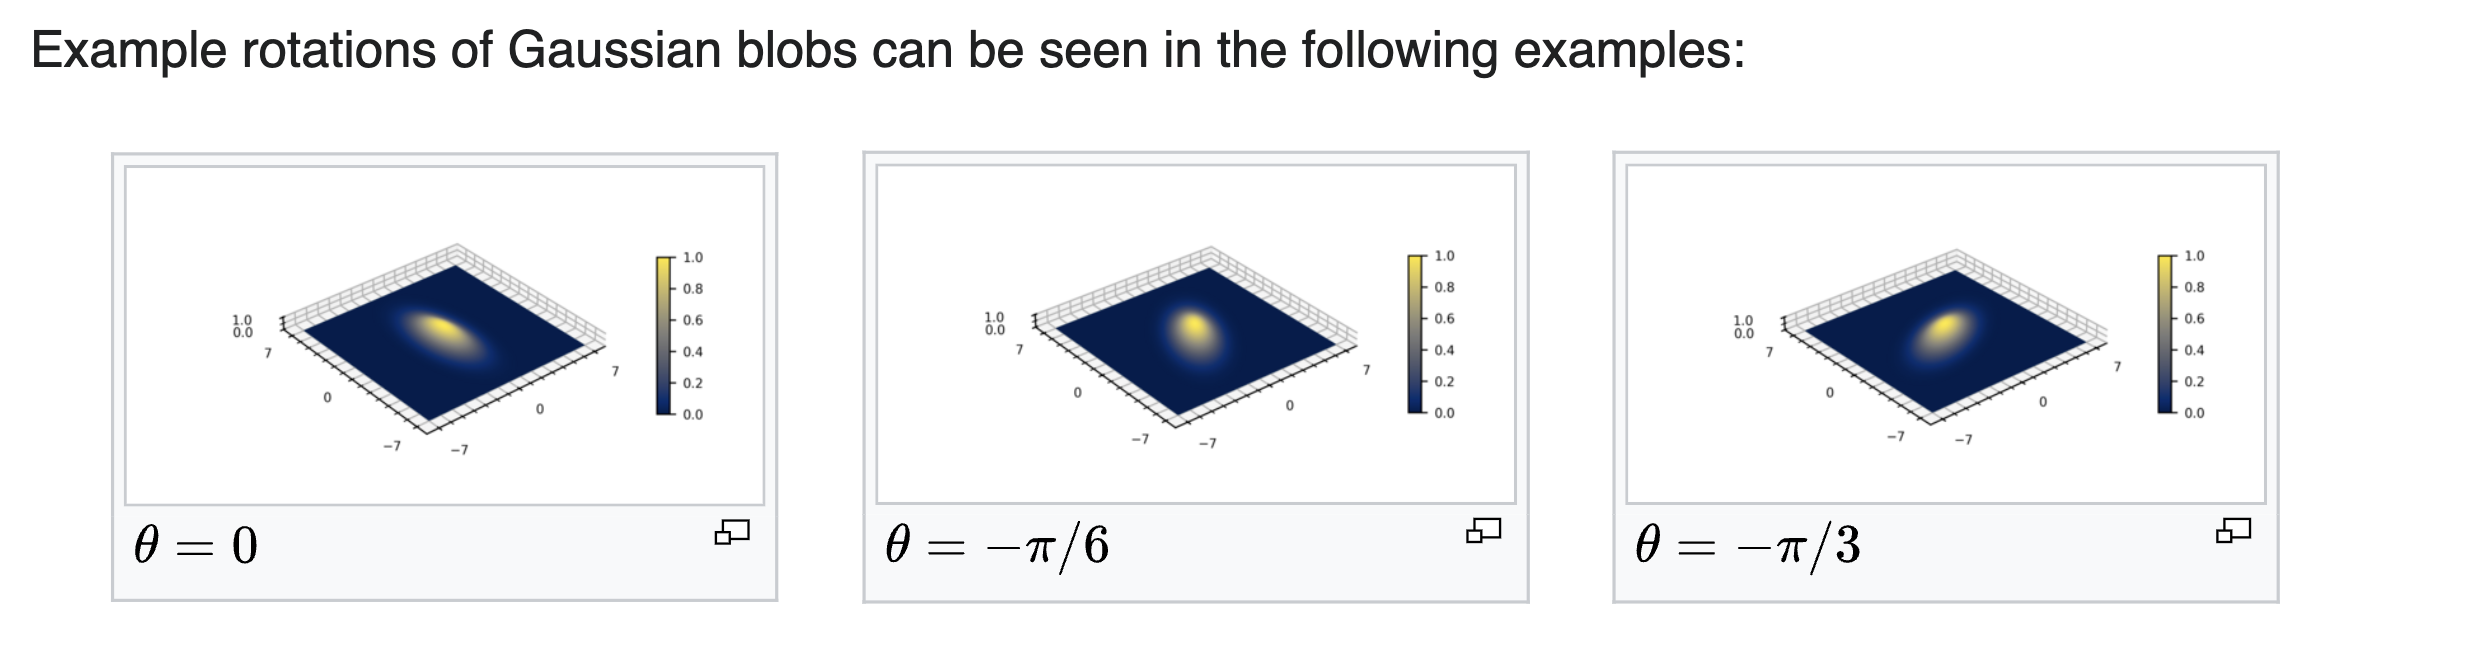
\includegraphics[width=1\linewidth]{theoretical-background/image/Gaussian.png}
    \caption{Gaussian Kernels results, \cite{wiki:gaussian}}
    
    \label{fig:gauss}
\end{figure}

The directions of Blobs have impactful on direct as Truth label for the Feature Map extractions from Image for Regression for counting. In crowd dense areas plots, high $\sigma$ variance and rotations may made the density maps blended and made wrong numberal feature. For Dynamic blobs, where $k_\sigma$ denotes a 2D Gaussian kernel with bandwidth $\sigma$, and $\ast$ represents the 2D convolution operation, the density map can be obtained by convolving the dot annotations with the Gaussian kernel. This is equivalent to placing a Gaussian distribution at each annotated point, leading to the following formulation for the density map:

\[
Y(p) = \sum_{\{p' \mid D(p') = 1\}} \mathcal{N}(p \mid p', \sigma^2 I),
\]

where $p$ and $p'$ are pixel locations in the image, and $\mathcal{N}(p \mid \mu, \Sigma)$ denotes the multivariate Gaussian distribution with mean $\mu$ and covariance $\Sigma$. In this setup, $D(p') = 1$ indicates the presence of a dot annotation at location $p'$.

In adaptive kernel approaches, the bandwidth $\sigma$ of the Gaussian kernel varies across the image depending on contextual cues such as local crowd density \cite{zhang2015cross} or scene perspective \cite{zhang2016single}. The crowd counting model is then trained using pairs of images and their corresponding density maps as ground truth.

\subsection{Dynamic Convolutional}

The Squeeze-and-Excitation (SE) block strengthens convolutional neural networks by allowing them to adaptively recalibrate channel-wise feature responses. This mechanism helps CNNs focus more on important features while suppressing less useful ones, improving their representational power with minimal computational overhead. By modeling inter-channel dependencies, SE blocks enhance feature discrimination and make the network more responsive to input-specific cues.

It achieved state-of-the-art performance in the ILSVRC 2017 classification challenge. Since then, SE blocks have been widely adopted in various architectures. SE-ResNet and SE-ResNeXt incorporate SE blocks into standard ResNet designs, yielding improved classification accuracy. EfficientNet uses SE blocks as part of its compound scaling strategy to achieve strong performance with fewer resources. MobileNetV3, designed for mobile and edge applications, also integrates SE blocks to improve efficiency and accuracy \cite{chen2020dynamic}

Dynamic Convolutions is an improvement over standard convolutional layers in deep neural networks. The main idea is to adapt the convolution kernel dynamically at each time step or spatial location based on the input features, without resorting to explicit attention mechanisms such as multi-head attention. It allow the model to adapt its filters based on the input without incurring the high computational cost of self-attention mechanisms. Unlike attention, the complexity remains linear with respect to the spatial dimensions. This makes dynamic convolutions particularly attractive for tasks such as image recognition and machine translation.

In contrast with traditional convolutions, dynamic convolutions utilize a set of $N$ convolution kernels $\{K_1, K_2, \dots, K_N\}$, each of shape $K_i \in \mathbb{R}^{C_{\text{out}} \times C \times k \times k}$. At each spatial position or time step (depending on the application), a weighted combination of these kernels is computed, where the weights depend on the input $X$. $w = f(X)$ be a function that computes the weights $w_i$ for $i = 1, \dots, N$, where $w_i$ is the finalize result of Squeeze and Exiting attention mechanism, mathematically, this mean that the $K_{\text{dyn}}$ is \textbf{Linearly Dependence} on other kernels, where it can be expressed as:  
\[w_i \geq 0, \quad \sum_{i=1}^N w_i = 1, K_{\text{dyn}} = \sum_{i=1}^N w_i K_i.
\]
This dynamic kernel is then applied in the usual convolution operation:
\[
Y = K_{\text{dyn}} * X.
\]

Importantly, the function $f(X)$ that produces the mixing weights can be implemented using global average pooling followed by a fully connected layer and softmax, i.e., where $\text{GAP}(X) \in \mathbb{R}^C$ and $W_{\text{fc}} \in \mathbb{R}^{N \times C}$. \cite{chen2020dynamic}
\[
w = \text{softmax}(W_{\text{fc}} \cdot \text{GAP}(X)),
\]

